\documentclass{article}
\usepackage{xcolor}
\usepackage{graphicx}
\usepackage{subcaption}
\usepackage{wrapfig}
\usepackage{booktabs}
\usepackage{multirow}
\usepackage[table]{xcolor}
\usepackage{colortbl}
\usepackage{longtable}
\title{Koustav Biswas}
\begin{document}
	\maketitle
	\section{INTRODUCTION}
	\textbf{Koustav Biswas} studies at \textit{BIT Mesra}.
	\textcolor{red}{Machine learning}
	\textit{This subject is \emph{interesting}}
 	is an important field of \underline{Artificial Intelligence}.
	It allows computers to learn patterns from data and make useful predictions.
	
	\definecolor{mycolor}{RGB}{100,200,30}
	\textcolor{mycolor}{Machine Learning}
	 is widely used in healthcare, finance, education, and transportation.
	 \colorbox{yellow}{	Good quality data helps Machine Learning models produce accurate and reliable results.}

	\fcolorbox{yellow}{red}{It is also used in applications such as computer vision and natural language processing.}
	The various types of ML Algorithms are {\small unsupervised},
	{\large supervised} and {\Large Reinforcement Learning}
	\begin{quote}
		\centering
		ML is what you need
	\end{quote}
	\section{Special Characters and Symbols}
	\$,\&,\%,\@@
	\section{Bullets and Numbering}
	\begin{itemize}
		\item NLP
		\item LLM
		\item LSTM
		\item Web Development
		\begin{enumerate}
			\item HTML
			\item CSS
			\item JS
		\end{enumerate}
	\end{itemize}
	\section{Citations Testing}
	Networking is the invisible blueprint of the modern digital world, turning isolated hardware into a cohesive global web of instant communication \cite{Shalini S}. By mastering routing protocols, firewall architecture, and packet flows, engineers can architect resilient systems that safely transport vast amounts of data across continents in mere milliseconds \cite{Koustav}. Utilizing online simulators bridges the gap between abstract theory and real-world deployment, allowing you to safely stress-test configurations and analyze traffic behaviors in a risk-free environment.
	\begin{thebibliography}{5}
		\bibitem{Shalini S}
		2025 IEEE Conference, Bio-watch, A AIOT Framework for ground water detection
		\bibitem{Koustav}
		2026 Springer Conference
	\end{thebibliography}
	
	\section{Image Demonstration}
	\ref{fig:ml} shows the flower
	\begin{figure}
		\centering
		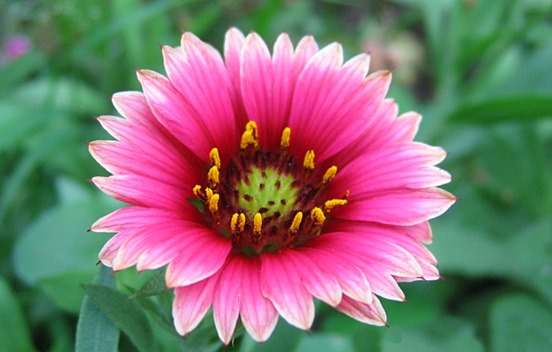
\includegraphics[width=1.0\textwidth]{flower.jpg}
		\caption{It is a flower}
		\label{fig:ml}
	\end{figure}
	
	\begin{figure}
		\centering
		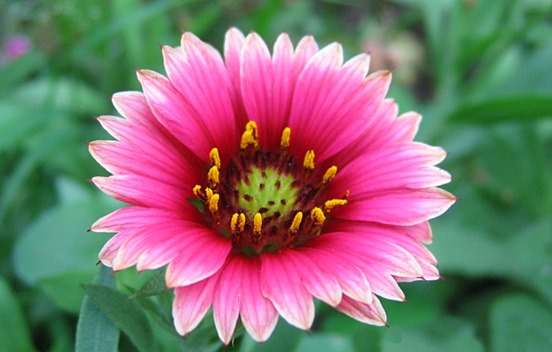
\includegraphics[angle=45]{flower.jpg}
		\caption{45 Degree flower}
		
	\end{figure}
		\begin{figure}
		\centering
		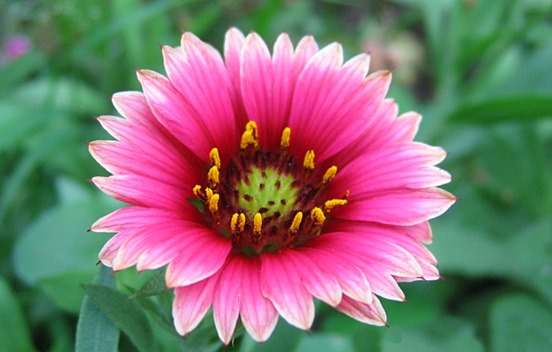
\includegraphics[angle=90]{flower.jpg}
		\caption{90 Degree flower}
	\end{figure}
	\section{side by side image}
	\begin{figure}
		\centering
		\begin{subfigure}{0.45 \textwidth}
			\centering
			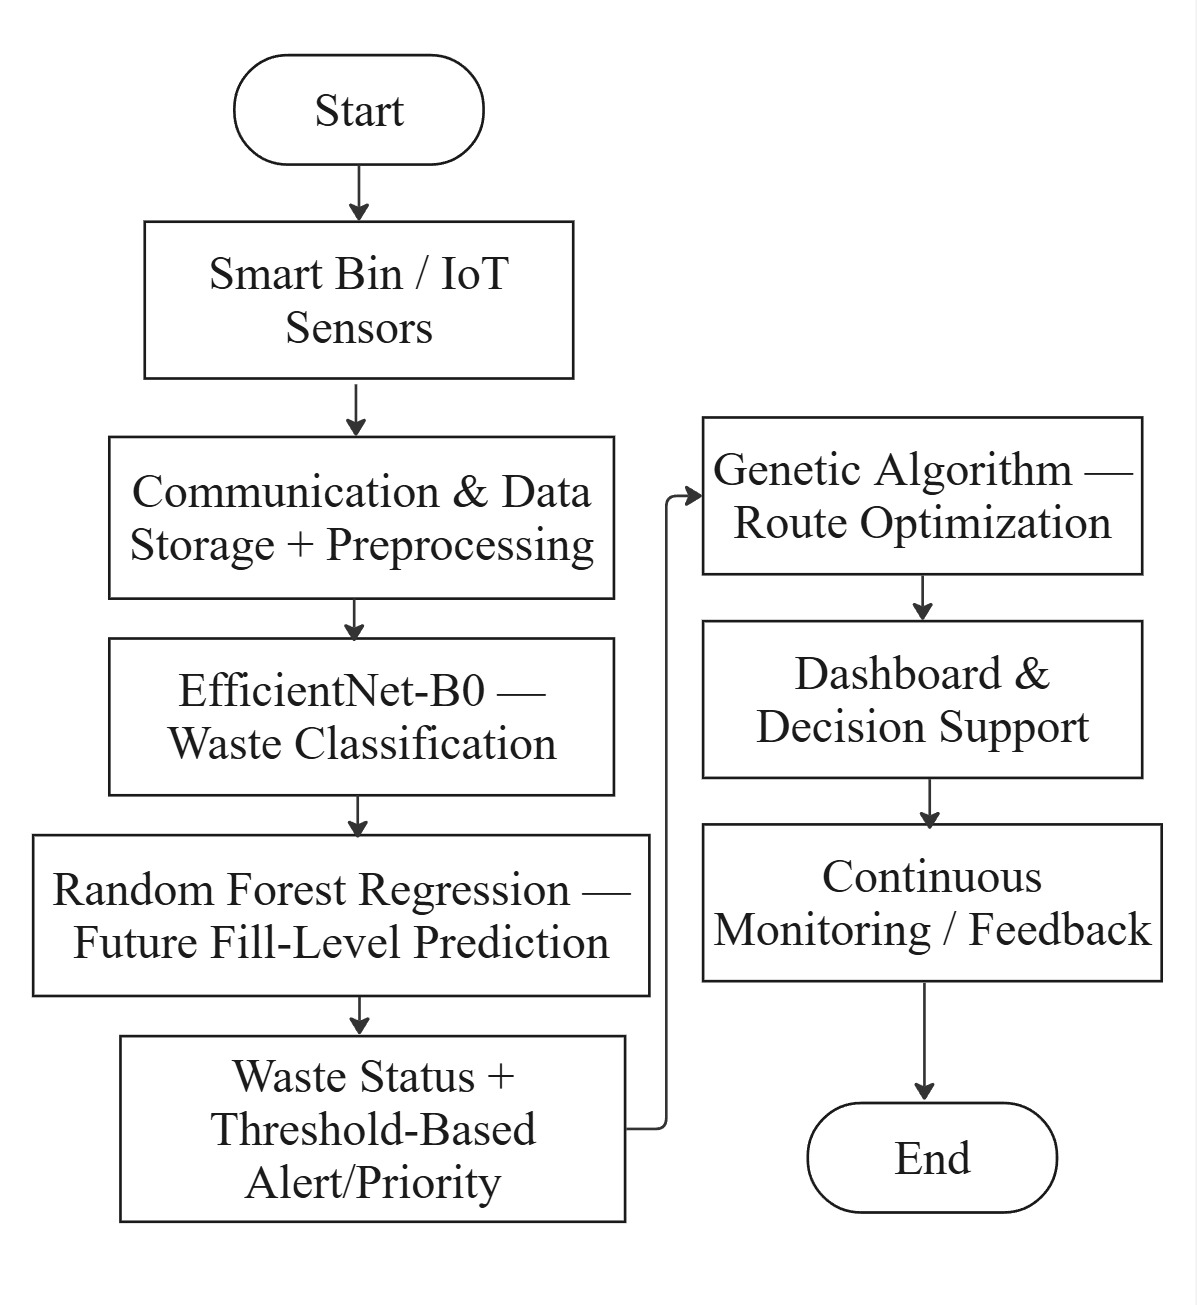
\includegraphics[width=\textwidth]{flow.jpg}
			\caption{First image}
		\end{subfigure}
		\hfill
		\begin{subfigure}{0.45 \textwidth}
			\centering
			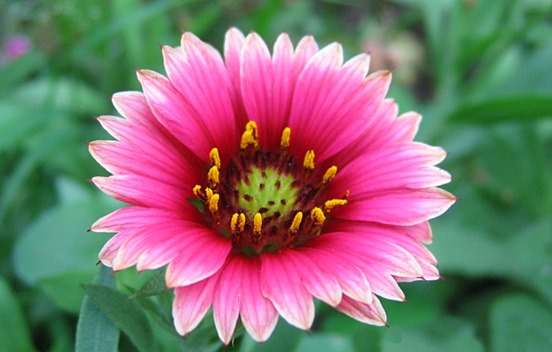
\includegraphics[width=\textwidth]{flower.jpg}
			\caption{second image}
		\end{subfigure}
		
		\begin{subfigure}{0.45 \textwidth}
			\centering
			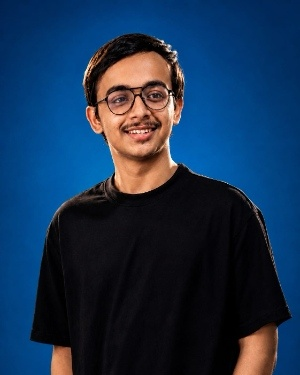
\includegraphics[width=\textwidth]{figure2.jpg}
			\caption{3rd figure}
		\end{subfigure}
		\hfill
		\begin{subfigure}{0.45\textwidth}
			\centering
			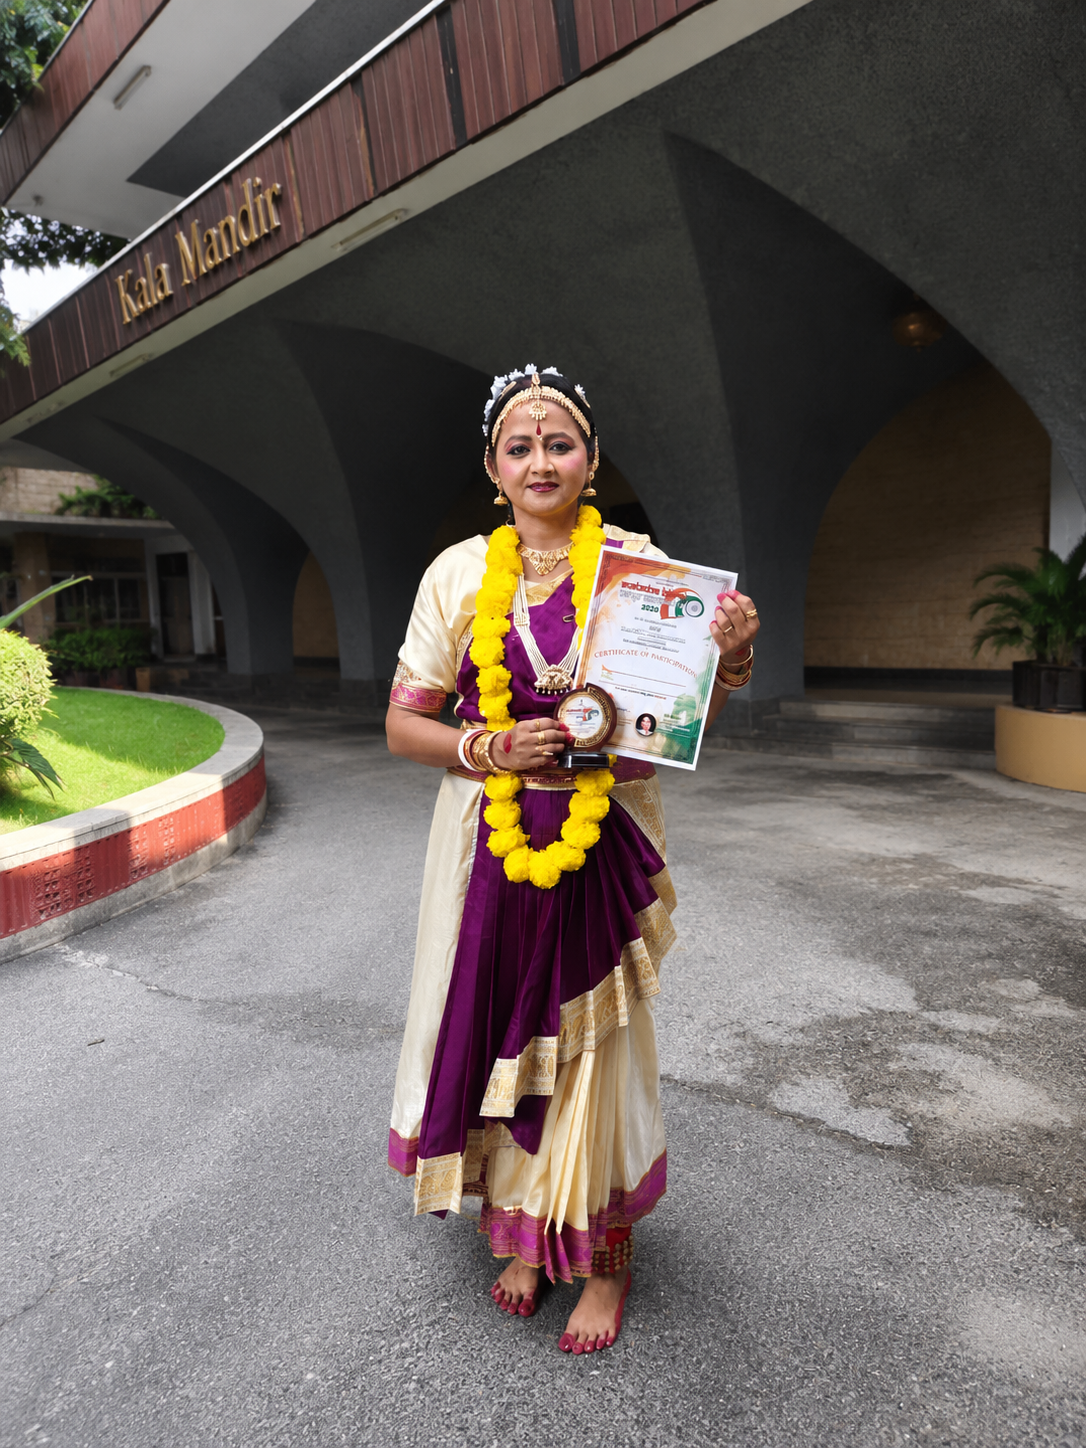
\includegraphics[width=\textwidth]{1.jpeg}
			\caption{4th figure}
		\end{subfigure}
		
	\end{figure}
	\section{Wrapping Text Around Images}
	\begin{wrapfigure}{l}{0.35\textwidth}
		\centering
		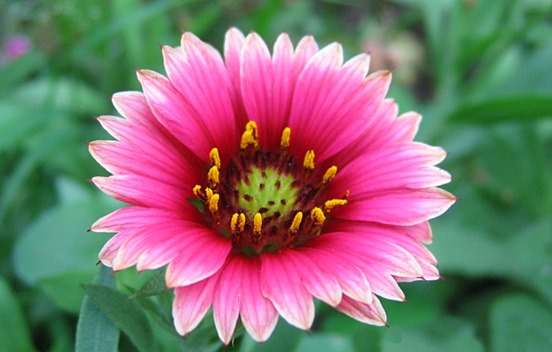
\includegraphics[width=0.3\textwidth]{flower.jpg}
		\caption{Machine Learning}
	\end{wrapfigure}
	
	Machine Learning is an important field of Artificial Intelligence.
	It allows computers to learn patterns from data and make useful predictions.
	Machine Learning is widely used in healthcare, finance, education, and transportation.
	Good quality data helps Machine Learning models produce accurate and reliable results.
	It is also used in applications such as computer vision and natural language processing.
	Changing r to l moves the image from the right side to the left side.
	When the image is placed on the left, the text flows around its right side.
	 The paragraph layout changes according to the position of the image.
	\section{Another Wrapping}
	\begin{wrapfigure}{r}{0.45 \textwidth}
		\centering
		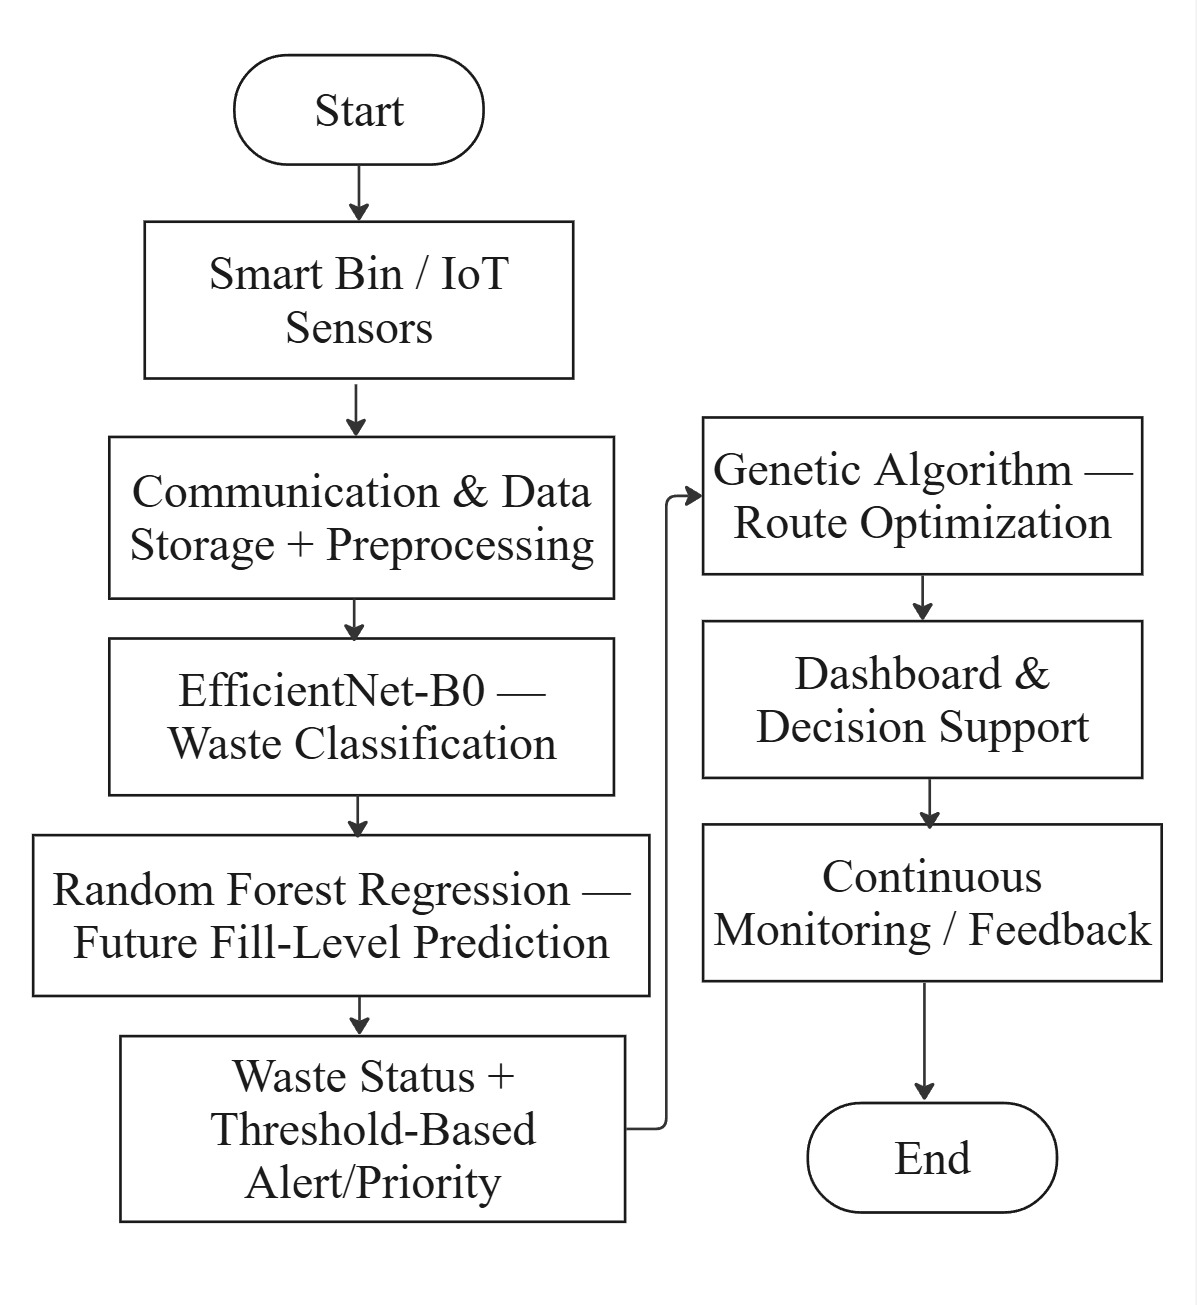
\includegraphics[width=0.3 \textheight]{flow.jpg}
		\caption{Flower}
	\end{wrapfigure}
		Good quality data helps Machine Learning models produce accurate and reliable results.
		It is also used in applications such as computer vision and natural language processing.
	\section{Four Images in a Grid}
	\begin{figure}[h]
		\centering
		
		% First row
		
		\begin{subfigure}{0.45\textwidth}
			\centering
			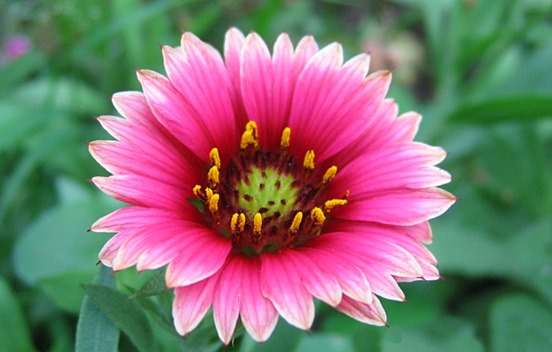
\includegraphics[width=\textwidth]{flower.jpg}
			\caption{First image}
		\end{subfigure}
		\hfill
		\begin{subfigure}{0.45\textwidth}
			\centering
			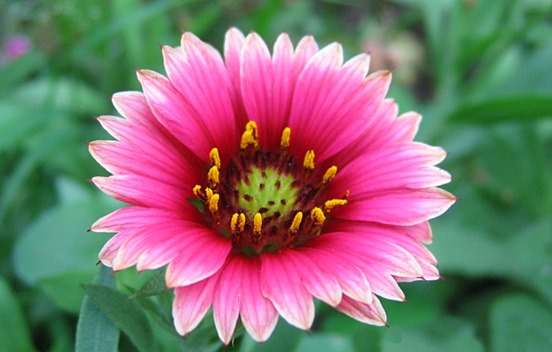
\includegraphics[width=\textwidth]{flower.jpg}
			\caption{Second image}
		\end{subfigure}
		
		\vspace{0.5cm}
		
		% Second row
		
		\begin{subfigure}{0.45\textwidth}
			\centering
			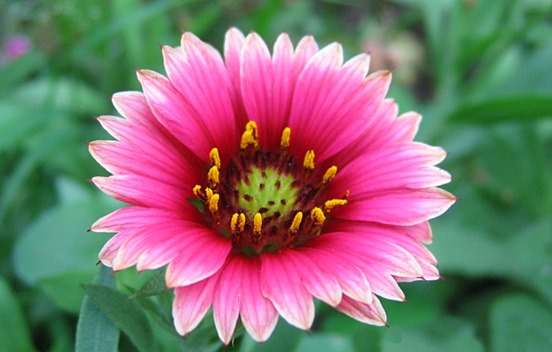
\includegraphics[width=\textwidth]{flower.jpg}
			\caption{Third image}
		\end{subfigure}
		\hfill
		\begin{subfigure}{0.45\textwidth}
			\centering
			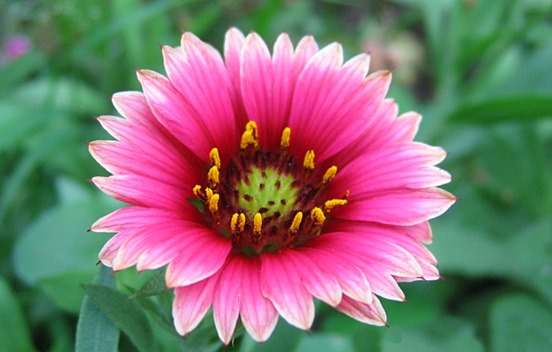
\includegraphics[width=\textwidth]{flower.jpg}
			\caption{Fourth image}
		\end{subfigure}
		
		\caption{Four images arranged in a 2-row, 2-column grid}
		\label{fig:grid}
		
	\end{figure}
	\section{Artificial Intelligence in Healthcare}
	Artificial Intelligence (AI) is transforming the healthcare sector by
	supporting doctors, improving diagnosis, and assisting in patient care.
	Machine Learning models can analyze large amounts of medical data and
	identify useful patterns. AI-based systems are also used in medical
	image analysis, disease prediction, and personalized treatment planning.
	
	% Technique 1: Full-width figure
	
	\begin{figure}[h]
		\centering
		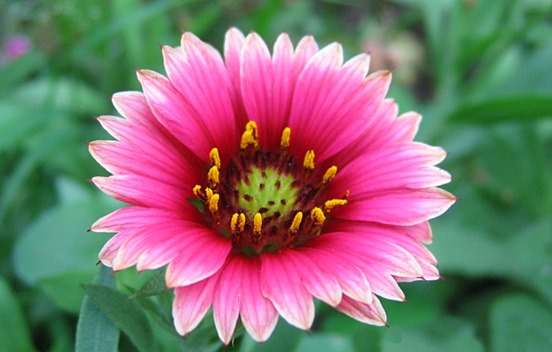
\includegraphics[width=0.9\textwidth]{flower.jpg}
		\caption{Applications of Artificial Intelligence in Healthcare}
		\label{fig:healthcare}
	\end{figure}
	
	Figure \ref{fig:healthcare} illustrates the role of AI in healthcare.
	Medical imaging and predictive analytics are important applications
	of these technologies.
	
	% Technique 2: Two side-by-side images
	
	\begin{figure}[h]
		\centering
		
		\begin{subfigure}{0.45\textwidth}
			\centering
			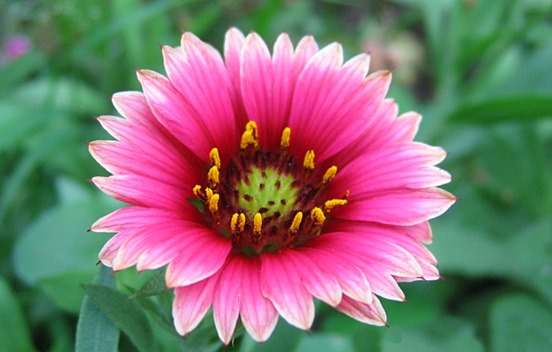
\includegraphics[width=\textwidth]{flower.jpg}
			\caption{AI-based diagnosis}
		\end{subfigure}
		\hfill
		\begin{subfigure}{0.45\textwidth}
			\centering
			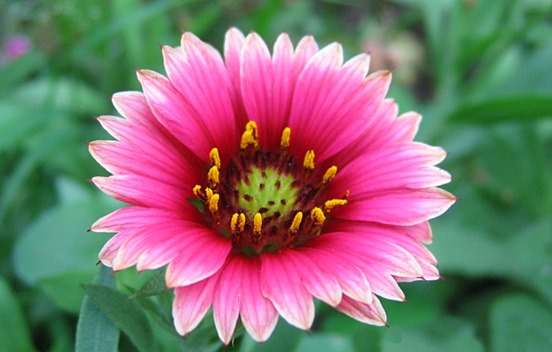
\includegraphics[width=\textwidth]{flower.jpg}
			\caption{Robotic assistance}
		\end{subfigure}
		
		\caption{Examples of AI applications in healthcare}
		\label{fig:applications}
	\end{figure}
	
	% Technique 3: Wrapped image
	
	\begin{wrapfigure}{r}{0.3\textwidth}
		\centering
		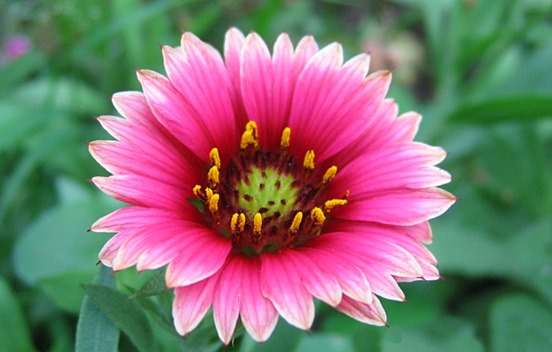
\includegraphics[width=0.27\textwidth]{flower.jpg}
		\caption{Medical AI}
	\end{wrapfigure}
	
	AI can also support remote healthcare services and assist medical
	professionals in making informed decisions. However, the quality of
	medical data, patient privacy, security, and ethical considerations
	must be carefully addressed.\\ Human supervision remains important when
	AI systems are used in clinical environments.
	
	% The full-width figure occupies most of the text width.
	% The subfigure environment places two images side by side.
	% The wrapfigure environment allows text to flow around an image.
	% Changing r to l moves the wrapped image from the right to the left.
		\section{Student Information}
	
	\begin{tabular}{|l|c|r|l|}
		\hline
		Name & Subject & Marks&cgpa \\
		\hline
		Koustav & Mathematics & 95&9.2 \\
		\hline
		Rahul & Physics & 88 &9.0 \\
		\hline
		Priya & Computer Science & 92&9.6 \\
		\hline
	\end{tabular}
	\section{Student Performance}
	
	Table \ref{tab:marks} presents the subjects, marks, and grades
	obtained by a student.
	
	\begin{table}[t]
		\centering
		
		\caption{Subject-wise Marks and Grades}
		\label{tab:marks}
		
		\begin{tabular}{lcc}
			\toprule
			Subject & Marks & Grade \\
			\midrule
			Mathematics & 95 & A+ \\
			Computer Science & 92 & A+ \\
			Physics & 85 & A \\
			English & 78 & B+ \\
			\bottomrule
		\end{tabular}
		
	\end{table}
	\iffalse
	Option	Meaning
	h	Here
	t	Top of the page
	b	Bottom of the page
	p	Separate page for floats
	!	Ask LaTeX to relax some placement restrictions
	\fi
	\section{Semester Result}
	
	\begin{table}[h]
		\centering
		
		\caption{Semester Result}
		\label{tab:semester}
		
		\begin{tabular}{lcc}
			\toprule
			
			\multicolumn{3}{c}{\textbf{Semester Result}} \\
			
			\midrule
			
			Subject & Marks & Grade \\
			
			\midrule
			
			Mathematics & 95 & A+ \\
			Computer Science & 92 & A+ \\
			
			\bottomrule
		\end{tabular}
		
	\end{table}
	\iffalse
	\label{tab:marks}	Creates a reference key
	\toprule	Adds a thick rule above the header
	\midrule	Adds a rule below the header
	\bottomrule	Adds a rule at the bottom
	\ref{tab:marks}	Displays the table number
	\fi
	
	\section{Department-wise Student Results}
	
	\begin{table}[h]
		\centering
		
		\caption{Department-wise Results}
		\label{tab:department}
		
		\begin{tabular}{l l c c}
			\toprule
			Department & Year & Students & Average Marks \\
			\midrule
			
			\multirow{2}{*}{CSE}
			& 1st Year & 60 & 85 \\
			& 2nd Year & 55 & 88 \\
			\midrule
			
			\multirow{2}{*}{ECE}
			& 1st Year & 58 & 82 \\
			& 2nd Year & 52 & 86 \\
			
			\bottomrule
		\end{tabular}
		
	\end{table}
	\section{Student Performance}
	
	\begin{table}[h]
		\centering
		
		\caption{Subject-wise Marks and Grades}
		\label{tab:marks}
		
		\begin{tabular}{lcc}
			\toprule
			
			\rowcolor{blue!20}
			Subject & Marks & Grade \\
			
			\midrule
			
			Mathematics & 95 & A+ \\
			
			\rowcolor{gray!15}
			Physics & 85 & A \\
			
			English & 78 & B+ \\
			
			\rowcolor{gray!15}
			Computer Science & 92 & A+ \\
			
			\bottomrule
		\end{tabular}
		
	\end{table}
	\section{Class Roll List}
	
	\begin{longtable}{c l c}
		
		\caption{Class Roll List} \\
		
		\toprule
		Roll No. & Name & Marks \\
		\midrule
		\endfirsthead
		
		\multicolumn{3}{c}%
		{{\tablename\ \thetable{} -- Continued from previous page}} \\
		
		\toprule
		Roll No. & Name & Marks \\
		\midrule
		\endhead
		
		\midrule
		\multicolumn{3}{r}{{Continued on next page}} \\
		\endfoot
		
		\bottomrule
		\endlastfoot
		
		1  & Koustav & 95 \\
		2  & Rahul & 88 \\
		3  & Priya & 92 \\
		4  & Amit & 81 \\
		5  & Sneha & 89 \\
		6  & Arjun & 76 \\
		7  & Riya & 94 \\
		8  & Rohit & 85 \\
		9  & Ananya & 91 \\
		10 & Vivek & 79 \\
		11 & Pooja & 87 \\
		12 & Aditya & 93 \\
		13 & Neha & 84 \\
		14 & Suman & 90 \\
		15 & Tanvi & 86 \\
		
	\end{longtable}
	\section{Machine Learning Results}
	
	Table \ref{tab:mlresults} presents the performance of different
	Machine Learning algorithms.
	
	\begin{table}[h]
		\centering
		
		\caption{Machine Learning Model Performance}
		\label{tab:mlresults}
		
		\begin{tabular}{lccc}
			\toprule
			
			\multicolumn{4}{c}{\textbf{Machine Learning Results}} \\
			
			\midrule
			
			\rowcolor{blue!20}
			Algorithm & Accuracy (\%) & Precision (\%) & Recall (\%) \\
			
			\midrule
			
			Logistic Regression & 91.2 & 89.5 & 86.8 \\
			
			\rowcolor{gray!15}
			Random Forest & 94.1 & 92.8 & 90.6 \\
			
			Support Vector Machine & 92.7 & 91.4 & 88.9 \\
			
			\rowcolor{gray!15}
			Decision Tree & 89.6 & 87.3 & 84.5 \\
			
			\bottomrule
		\end{tabular}
		
	\end{table}
	
	
	

\end{document}